% Source for the figure of PGMIndex (sec. 6.4): the points (A[i], i) of 14
% keys, covered by two segments whose lines predict each place within
% epsilon = 2 (the band); a search predicts the place of a key on the line
% of its segment and searches the window of the places within the error.
% Build: make figures (in ../build).
\documentclass[border=4pt]{standalone}
\usepackage[T1]{fontenc}
\usepackage{newpxtext,newpxmath}
\usepackage[varqu,varl,scaled=0.95]{zi4}
\usepackage{tikz}
% tikz-ads.tex: the TikZ styles shared by the figures of the memory of the
% manual, \input by each standalone figure: a cell of a vector (cell), the
% cell that an operation touches (touched), a free cell (free), a node of a
% linked structure (node), the labels of indices (index) and of variables
% (var), a pointer (ptr), and \cells and \indices to draw a row of cells.
\usetikzlibrary{arrows.meta,positioning,calc,fit,shapes.multipart}
\definecolor{adsTouched}{RGB}{214,196,236}
\definecolor{adsFree}{RGB}{236,236,236}
\tikzset{
  ads/.style={>={Stealth[length=2mm]},font=\small,
              every node/.append style={inner sep=0pt}},
  cell/.style={draw,minimum width=7mm,minimum height=7mm,
               font=\small\ttfamily,outer sep=0pt},
  touched/.style={cell,fill=adsTouched},
  free/.style={cell,fill=adsFree,text=black!45},
  node/.style={draw,rounded corners=1pt,minimum width=8mm,
               minimum height=6mm,font=\small\ttfamily},
  index/.style={font=\scriptsize\ttfamily,text=black!60},
  var/.style={font=\small\itshape},
  ptr/.style={->,thick}
}
% \cells{name}{x,y}{list}: a row of cells, the first at (x,y), named
% name-0, name-1, ...; each item is text/style, the style one of cell,
% touched and free (e.g., {a/cell,e/touched,/free})
\newcommand{\cells}[3]{%
  \foreach \v/\s [count=\i from 0] in {#3}
    \node[\s] (#1-\i) at ($(#2)+(\i*7mm,0)$) {\v};}
% \indices{name}{n}: the indices 0 .. n-1 under the cells of name
\newcommand{\indices}[2]{%
  \foreach \i in {0,...,\numexpr#2-1\relax}
    \node[index,below=1.2mm of #1-\i] {\i};}

\usetikzlibrary{decorations.pathreplacing}
\begin{document}
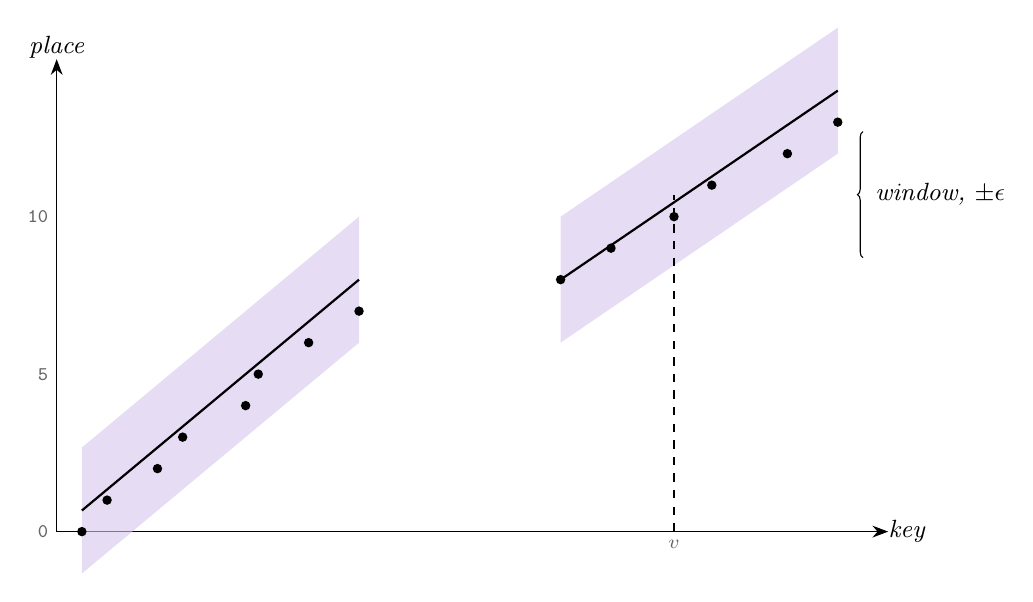
\begin{tikzpicture}[ads,x=1.6mm,y=4mm]
  \draw[->] (0,0) -- (66,0) node[right,var] {key};
  \draw[->] (0,0) -- (0,15) node[above,var] {place};
  % the first segment: keys 2 .. 24, slope 0.33
  \fill[adsTouched,opacity=0.6] (2,-1.33) -- (24,6) -- (24,10) -- (2,2.67) -- cycle;
  \draw[thick] (2,0.67) -- (24,8);
  % the second segment: keys 40 .. 62, slope 0.27
  \fill[adsTouched,opacity=0.6] (40,6) -- (62,12) -- (62,16) -- (40,10) -- cycle;
  \draw[thick] (40,8) -- (62,14);
  \foreach \x/\y in {2/0,4/1,8/2,10/3,15/4,16/5,20/6,24/7,
                     40/8,44/9,49/10,52/11,58/12,62/13}
    \fill (\x,\y) circle (0.6mm);
  \foreach \y in {0,5,10}
    \node[index,left=1mm] at (0,\y) {\y};
  \draw[dashed] (49,0) -- (49,10.7);
  \node[index,below=1mm] at (49,0) {$v$};
  \draw[decorate,decoration={brace,amplitude=2pt}] (64,8.7) -- (64,12.7)
    node[midway,right=1.5mm,var] {window, $\pm \epsilon$};
\end{tikzpicture}
\end{document}
